% <<< Preamble
\documentclass[a4paper, 12pt]{article}
\usepackage[french]{babel}
\usepackage{fontspec}
\usepackage{hyperref}
\usepackage{lmodern}
\renewcommand*\familydefault{\sfdefault} %% Only if the base font of the document is to be sans serif
\linespread{1.05} 
\usepackage{fancyhdr}
\usepackage[dvipsnames]{xcolor}
\usepackage{xspace}
\usepackage[head=2cm,top=1cm,left=2cm,right=2cm]{geometry}
\usepackage{lastpage}
\usepackage{graphicx}
\usepackage[bottom]{footmisc}
\newcommand{\verif}{\textcolor{red}{\textbf{??}}\xspace}
\newcommand{\todotext}{\textcolor{red}{\textbf{TODO}}\xspace}

\geometry{
  a4paper,
  left=20mm,
  right=20mm,
  bottom=2cm,
}
\hyphenation{gé-né-ral}

\usepackage[framemethod=TikZ]{mdframed}

\usepackage{amssymb}% http://ctan.org/pkg/amssymb
\usepackage{pifont}% http://ctan.org/pkg/pifont
\newcommand{\cmark}{\ding{51}}%
\newcommand{\xmark}{\ding{55}}%
\newcommand{\done}{{\color{OliveGreen}\rlap{$\square$}{\raisebox{2pt}{\large\hspace{1pt}\cmark}}}%
\hspace{-2.5pt}}
\newcommand{\wontfix}{\rlap{$\square$}{\large\hspace{1pt}\xmark}}
\newcommand{\todosquare}{{\color{Red}{\boldmath $\square$}}}

\newcommand{\tache}[1]{
\mdfsetup{linecolor=Red, linewidth=2pt, roundcorner=5pt }
  \begin{flushright}
    \begin{minipage}{4cm}
  \begin{mdframed}
    \begin{itemize}
      \item[\todosquare] \textbf{#1}
    \end{itemize}
  \end{mdframed}
    \end{minipage}
  \end{flushright}
}

\newcommand{\fini}[1]{
\mdfsetup{linecolor=OliveGreen, linewidth=2pt, roundcorner=5pt }
  \begin{flushright}
    \begin{minipage}{4cm}
  \begin{mdframed}
    \begin{itemize}
      \item[\done] \textbf{#1}
    \end{itemize}
  \end{mdframed}
    \end{minipage}
  \end{flushright}
}

\pagestyle{fancy} 
\fancyhf{}
\renewcommand{\headrulewidth}{0pt}
%\renewcommand{\footrulewidth}{0.5pt}
\fancyfoot[R]{version du \today}
\fancyfoot[C]{\thepage / \pageref{LastPage}}
% >>>

\begin{document}

\begin{center}
  {\Large Contenu du site de documentation JupytherHub}\\[3ex]
\end{center}

% <<< intro
\begin{center}
\rule{.5\textwidth}{1pt}
\end{center}

Ci-dessous se trouve la table des matières du site
\url{https://jhub.cnam.fr/doc/}. Je propose d'utiliser ce document Latex pour
en organiser la rédaction. Ce document est versionné avec git, déposé sur le
gitlab.cnam.fr. Il se trouve dans un dossier non transformé par Jekyll
(\verb+_redaction+). 

Les sections ci-dessous correspondent à des grandes parties du site, qui
contiennent une ou plusieurs pages. Il peut y avoir une page pour présenter la
section. Voir la section Brainstorming en fin de document, pour mémoire.\\

Dans la réunion de travail du 13 novembre 2020, il a été décidé que le site
était surtout destiné à nos collègues enseignants. Pour les auditeurs, ce sera
surtout les enseignants qui leur communiqueront des liens et de la documentation
Jupyter existante. Ces références sont à organiser dans la section Liens, dans
une sous partie/une page dédiée. À partir du contenu rédigé de ce site, un
document papier pourra être rédigé et mis en ligne, de façon à promouvoir le
projet auprès des instances et servir de bases aux futurs appels à projet (cf la
"fiche de synthèse" débutée sur Overleaf).

Le calendrier de rédaction discuté le 13 novembre 2020 fixait une date de
"sortie" de ce site pour le début du 2e semestre 2020-21 (un {\em go-live},
dit-on dans le jargon de la start-up nation\footnote{de notre président marcheur
préféré, que ses pas soient tapissés de feuilles de roses}), c'est-à-dire le 8
février 2021. Je (Raphaël) propose donc de faire un point d'étape un mois avant, le 8
janvier 2021.

La répartition de la rédaction des pages est indiquée ci-dessous. On peut en
rediscuter, mais il faudrait valider rapidement ces responsabilités : je propose
que la dernière version de ce document commitée dans le dépôt avant le 4
décembre inclus serve de référence. Une fois qu'une tâche est finie, il suffit
de remplacer \verb+\tache+ par \verb+\fini+.

\begin{center}
\rule{.5\textwidth}{1pt}
\end{center}
% >>>

\section{Accueil}

Une page, avec un message clair pour présenter JupyterHub rapidement et inviter à le découvrir avec les différentes sections (liens).
Le texte de Josselin peut servir de base, évidemment : \url{https://formation.cnam.fr/projet-6-plate-forme-d-analyse-des-donnees-competences-et-employabilite-par-la-pratique-1204533.kjsp}

\tache{Josselin}

\section{C'est quoi ?}
Une page, avec 3 parties :
\begin{itemize}
\item Présentation de l’interface
\item Support multimédia
\item Exportations multiples 
\end{itemize}

\tache{Raphaël}

\section{À quoi ça sert ?}

\subsection{Manipulation}
Ce point n'est plus très clair pour moi, j'espère qu'il le sera pour d'autres.
\tache{Chloé ?}

\subsection{Calcul, programmation}
Des exemples de carnets pour l'apprentissage de la programmation ?
\tache{Simon}

\subsection{Support pédagogique}
Comment l'utiliser, de façon simple (TP à trous ?) ou de façon complexe (comment rédiger un poly complet et le convertir en \LaTeX\, et pdf, cf poly de Josselin).

\tache{Chloé}

\section{Utilisation au CNAM}
Une page par sous-section environ

\subsection{JupyterHub et Moodle}
L'intégration du login, quelques éléments
\tache{Rafik}

\subsection{JupyterLab}
Une page rapide pour présenter ce mode.
\tache{Simon}

\subsection{Règles d’usage}
Des détails sur les "bonnes pratiques"
\tache{Rafik}

\subsection{FAQ (questions fréquentes)}
Si on a déjà une liste de questions fréquentes. Sinon, à cacher au début.

\subsection{Liste de packages - fiche technique}
la liste de ce qui existe actuellement, la notion d'images customisées, comment demander des ajouts, etc.
\tache{Rafik}

\section{Liens}

Une page, avec une partie dédiée à "ce que les enseignants pourront distribuer
comme doc de référence à leurs élèves".

\tache{Josselin}

\section{Contact}
Une page, avec l'essentiel, c'est-à-dire le mail de Rafik :-)

\fini{Raphaël}

\section{Markdown kitchen sink}

Une page d'aide déjà écrite, à déplacer dans un coin. Mais pour le moment elle
peut servir de référence pour formater le contenu (en markdown).

\begin{center}
\rule{.5\textwidth}{1pt}
\end{center}
\section*{Brainstorming}

\begin{figure}[!ht]
  \centering
  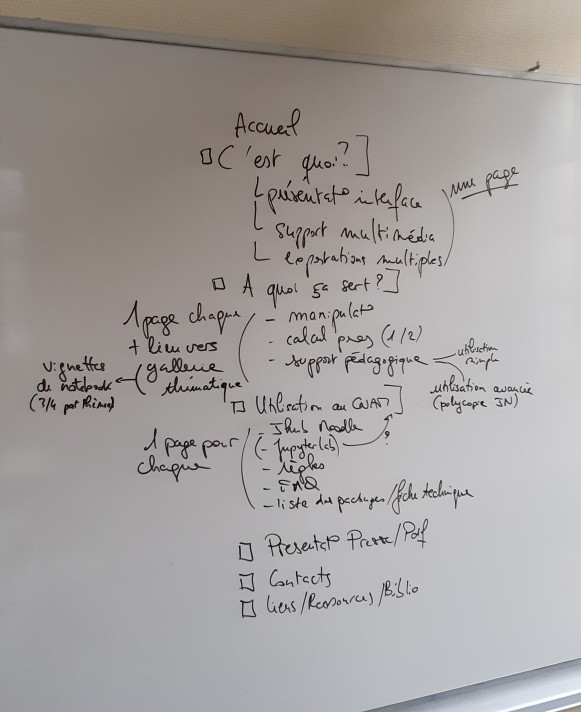
\includegraphics[width=.4\textwidth]{brainstorm.jpg}
  \caption{Une bien belle séance de travail. 6 février 2020, 17h38}
\end{figure}

\end{document}
% vim: set fdm=marker fmr=<<<,>>> fdl=0:fdc=2
